%% ------------------------------------------------------------------------- %%
\chapter{Metodolologia e Processamento}
\label{cap:processamento}

Esse capítulo apresenta como as teorias do capítulo anterior foram utilizadas para obtenção 
dos resultados que serão discutidos no próximo capítulo.

%% ------------------------------------------------------------------------- %%
\section{Conjunto de Dados}
\index{Conjunto de Dados}
\label{sec:dados}

Os dados utilizados foram os dados do catálogo \gls{isc}-\gls{gem} (REFERENCIA) 
para a América do Sul e 
os dados do \gls{bsb} (REFERENCIA) para o Brasil.

O dados são texto e formatados em arquivos de \gls{csv}-UTF-8.

%% ------------------------------------------------------------------------- %%
\subsection{Catálogo ISC-GEM}
\index{Conjunto de Dados!ISC-GEM}
\label{sec:data_source}

O catálogo \gls{isc}-\gls{gem} versão XXX possui licença CC-BY-SA e é fruto da redeterminação de parâmetros
dos terremotos com os dados disponíveis no ISC-GEM e de um detalhado estudo para que ao menos um valor de
magnitude $\gls{sym:Mw}$ estivesse disponível com incertezas.

\subsection{Boletim Sísmico Brasileiro}
\index{Conjunto de Dados!BSB}
\label{sec:data_source2}

O \gls{bsb}, versão 2013.08 possui licença CC-BY e é fruto do esforço de compilação de
dados e determinação de epicentros e magnitudes que contou com a colaboração de várias instituições
como o \gls{obsis} da \gls{unb}, o \gls{ipt}, a \gls{unesp}, a \gls{ufrn} liderados pelo \gls{iag} da \gls{usp}.


%% ------------------------------------------------------------------------- %%

\section{Ferramentas}
\index{Ferramentas}
\label{sec:ferramentas}

As ferramentas utilizadas para as análises e cálculos apresentados nesse texto
foram de código aberto.
Utilizou-se o Latex para a edição do texto, o software de processamento de dados
geoespacial QGIS, o console do Linux BASH, a IDE Eclipse, o git/GitHub para o controle de versao,

O iPython como console interativo, a MatplotLib e Basemap para o gráficos, 
a SciPy para um conjunto de funções científicas e estatísticas, a shapely e gdal
para lidar com objetos com atributos geométricos.


%% ------------------------------------------------------------------------- %%
\subsection{Linguagens de Programação}
\index{Linguagens de Programação}
\label{sec:linguagens}

A principal linguagem de programação utilizada foi Python.

Os códigos-fonte dos modelos de Woo e de Helmstetter foram providos pelos autores
e estão em Fortran. O método de Frankel estava disponível em Python.


%% ------------------------------------------------------------------------- %%
\subsection{Programas de Computador}
\index{Ferramentas!programas}\index{software}
\label{sec:software}

O programa mais comum para esse tipo de análise costuma ser o CRISIS nas suas mais diversas
versões. Como nesse trabalho a opção foi por código aberto, poderia ter se optado pelo 
\gls{opensha} que é escrito em Java.

A intenção no entanto foi provar o conjunto de tecnologias mantido pela Fundação \gls{gem}
que para o cálculo de ameaça e rísco sísmico que é o \gls{oq}.

O código do \gls{oq} está abertamente disponível para consulta e clonagem no GitHub.

O ecossistema do \gls{oq} é ilustrado na figura a seguir:

\begin{figure}[!h]
  \centering
  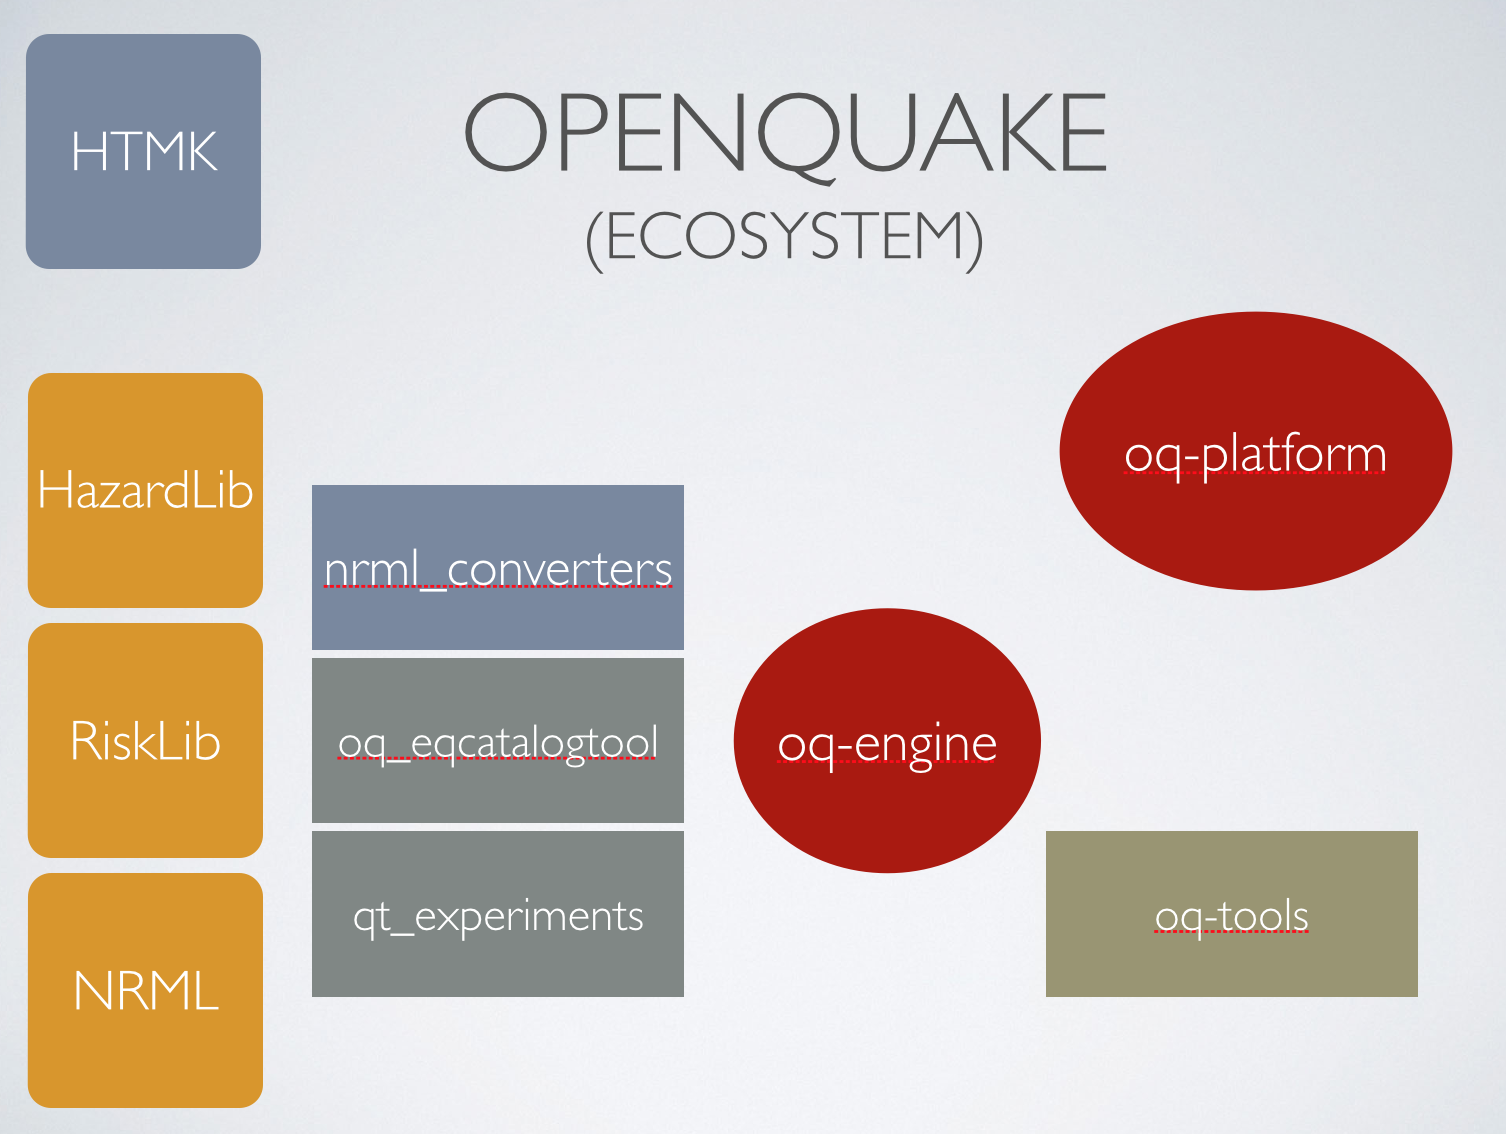
\includegraphics[width=.80\textwidth]{oq_ecosystem} 
  \caption{Ecossistema de módulos, bibliotecas e utilitários do OpenQuake}
  \label{fig:oq} 
\end{figure}

O destaque em vermelho na figura \ref{fig:oq} fica para o \gls{oqe} que executa as simulações de cada tronco da
arvore-lógica e as usa para calcular o cenário de risco e armazenar o resultado.
Faz isso distribuindo o processamento em tarefas e permitindo escalar o cálculo.

A \gls{oqp} permite interagir com os dados armazenados e gerenciados na nuvem, como catálogos, 
falhas, dados de esforços, fontes sismogênicas e suas geometrias usados em cálculos de ameaça/risco.
Permite também interagir com o resultado do cálculo, visualizando mapas de ameaça e curvas de intensidade.

%% ------------------------------------------------------------------------- %%
\subsection{Bibliotecas de Funções}
\index{ferramentas!bibliotecas}
\label{sec:bibliotecas}

Em amarelo na figura \ref{fig:oq} está biblioteca a \gls{hl} que contém toda lógica e ciência para o cálculo de ameaça,
como os tipos de fontes sísmogênicas, as \gls{mfd}, as \glspl{gmpe}, etc. 

Está também a \gls{rl}
que contém os modelos de vulnerabilidade e exposição para a análise de risco. 

E por último,
a \gls{nrml} que é a sintaxe da linguagem de representação das árvores-lógicas, fontes sísmicas e
resultados, como mapas de risco, espectro de alguma medida de intensidade, etc. 


%% ------------------------------------------------------------------------- %%
\subsection{Implementações e Novos Códigos}
\index{Implementações e novos códigos }
\label{sec:implementacao}

Incluido no suporte da Fundação \gls{gem} está a manutenção de um Comitê Científico
que desenvolve ferramentas auxiliares adicionais como conversores, ferramentas para trabalho com 
o catálogo, ferramentas gráficas, entre outras para interação com o
\gls{oq} como pode ser visto na figura \ref{fig:oq} em azul, cinza e bege.

Uma dessas ferramentas em especial é o \gls{hmtk} que facilita todo o processo de modelagem da \gls{psha}
como a remoção de agrupamentos, a caracterização de zonas sísmicas,  
a visualização da evolução da taxa de sismicidade, a análise da magnitude de completude e
estimativa do valor-b.

O \gls{hmtk} já trazia um módulo para trabalhar com a sismicidade que usava as \gls{smoothing}
implementando o método de Frankel, 1995 (REFERENCIA). E é na \gls{hmtk} que se pretende
contribuir com a implementação dos métodos de Woo e de Helmstetter.
 
%% ------------------------------------------------------------------------- %%
\section{Pré-Processamento}
\index{pré-processamento}
\label{sec:pre_processamento}

Para aplicar as \gls{smoothing} no conjunto de dados é necessário alguns primeiros passos.
É disso que trata essa seção.


%% ------------------------------------------------------------------------- %%
\subsection{Controle de Qualidade}
\index{pre-processamento!controle de qualidade}
\label{sec:qualicontrol}

A primeira coisa a se fazer no conjunto de dados é uma primeira checagem da qualidade.

Nessa hora é preciso observar se não há pontos com coordenadas erradas, invertidas, faltando valores de dias ou horas.

É recomendado também fazer uma varredura em busca de artefatos no catálogo (REFERENCIA CORSSA).
Isso é feito com, por exemplo, um histogramas do dia da semana da ocorrencia dos tremores em busca
de algum descréscimo em fins de semana que seriam um provável indicativo de contaminação do catálogo 
por atividade de pedreiras. Outros exemplos são fazer um histograma para estimar a distribuição 
do horário de ocorrência durante o dia, ou mesmo da profundidade para estimar a resolução do catálogo
nesse quesito.

\begin{figure}[H]
  \centering
  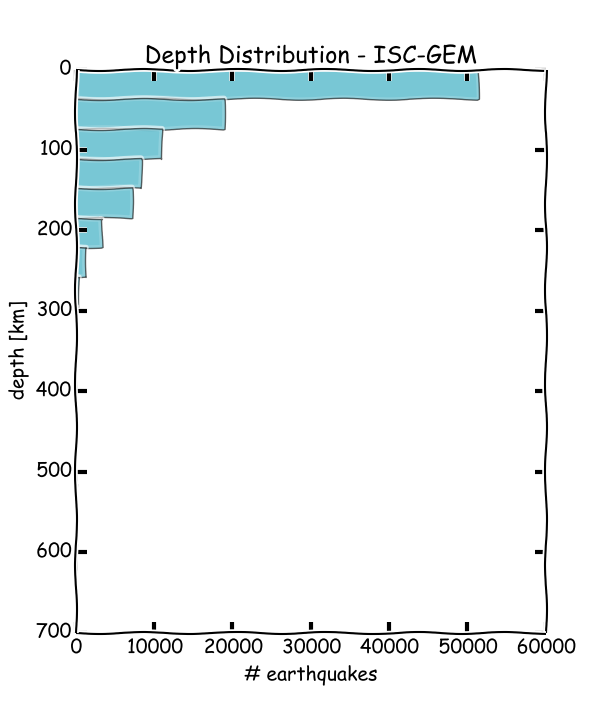
\includegraphics[width=.50\textwidth]{dep_sa_hist} 
  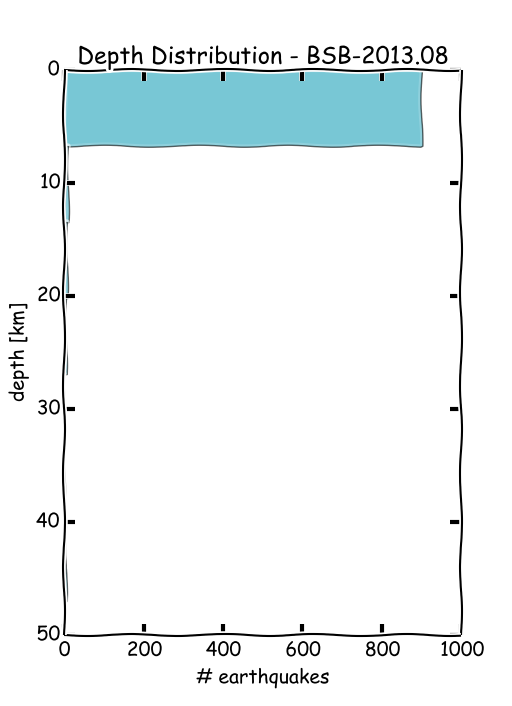
\includegraphics[width=.42\textwidth]{dep_br_hist} 
  \caption{Histogramas da Profundidade (em Km) dos Tremores}
  \label{fig:qc_dep_hist} 
\end{figure}



%% ------------------------------------------------------------------------- %%
\subsection{Remoção de agrupamentos}
\index{remoção de agrupamentos}\index{declustering}
\label{sec:declustering}

A maior parte dos modelos de sismicidade estudados aqui assumem que a ocorrência de
tremores segue um processo de Poisson.

Mas sabe-se que os predecessores e sucessores de tremores principais não são independentes.
E o aumento do número de sismos pouco antes e pouco depois de um grande tremor contamina
o catálogo com mais sismos do que seriam realmente esperados se fossem independentes.

Existem outros modelos que usam exatamente essa variação das taxas de sismicidade com o tempo
para fazerem projeções de curto-prazo.

O processo de remoção de agrupamentos (\emph{declustering}) REFERENCIA CORSSA busca
dentro de uma janela, de espaço-tempo como função da magnitude, os sismos e os considera como um único
sismo mais expressivo removendo os demais.

Aqui o processo de remoção de agrupamentos foi feito pela técnica de Reasemberg (REFERENCIA) com parâmetros
(XXXX).

%% ------------------------------------------------------------------------- %%
\subsection{Conversão de Magnitudes}
\index{magnitudes!conversão}
\label{sec:mag_conv}

Para que a magnitude dos tremores possam ser analizadas em termos do momento sísmico e do 
tamanho da ruptura que geram é preciso que os sismos do catálogo apresentem pelo menos um valor
\gls{Mw} para a magnitude.

No catálogo do ISC-GEM isso é assunto resolvido, mas no caso do \gls{bsb} a maior parte das magnitudes
são regionais $m_R$ que se assemelham às magnitudes $m_b$ ou magnitudes estimadas a partir de dados
macrossísmicos. Nos dois casos é preciso avaliar funções que relacionem os vários valores de magnitude
e \gls{Mw}.

As relações de magnitude usadas no \gls{bsb} nesse trabalho foram:

bls

bla

bal



%% ------------------------------------------------------------------------- %%
\subsection{Análise da Magnitude de Completude}
\index{Magnitude de Completude}
\label{sec:completeness}

O método disponível no \gls{hmtk} é o de Stepp, 1972 (REFERENCIA). Que permite
obter uma tabela de completude do catálogo.

FIGURA


EXPLICAR


%% ------------------------------------------------------------------------- %%
\section{Frankel, 1995}
\index{processamento!Frankel}
\label{sec:proc_frankel}

Para o processamento pelo método de Frankel, utilizou-se o catálogo com os agrupamentos removidos,
e uma distãncia de correlação de 150km devido à escala aplicada no contexto brasileiro.

%% ------------------------------------------------------------------------- %%
\section{Woo, 1996}
\index{processamento!Woo}
\label{sec:proc_woo}

O processamento pelo método de Woo também foi feito com a remoção dos agrupamentos no catálogo.

A largura de banda dependente da magnitude é ajustada pelo próprio método.
A figura~\ref{fig:woo_b} apresenta a ajuste para o \gls{bsb}:

\begin{figure}[H]
  \centering
  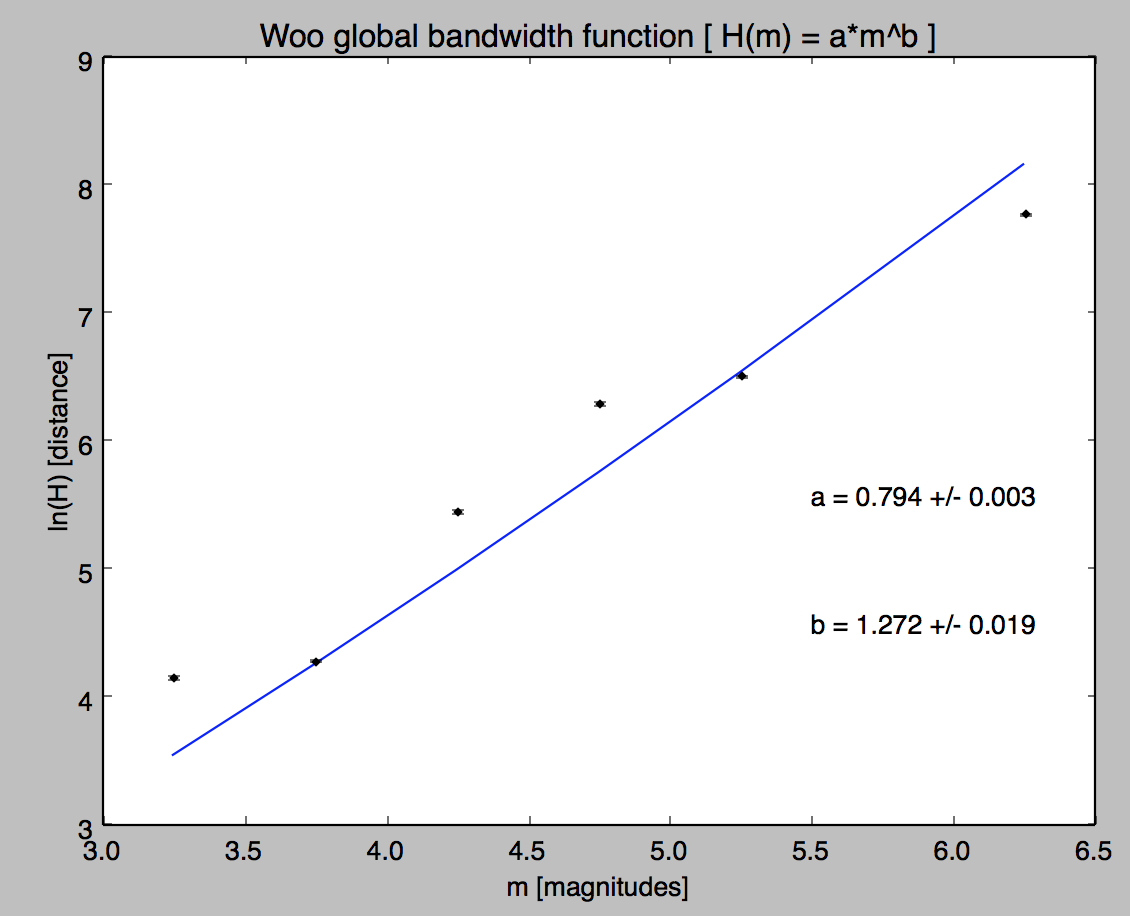
\includegraphics[width=.80\textwidth]{woo_bandwidth} 
  \caption{Ajuste da largura de banda para o método de Woo1996}
  \label{fig:woo_b} 
\end{figure}

Esse ajuste é consistente com os ajustes apresentados por Beauval (REFERENCIA)
para a França e Noruega.
 

%% ------------------------------------------------------------------------- %%
\section{Helmstetter, 2012}
\index{processamento!Helmstetter}
\label{sec:proc_helmstetter}

Utilizou-se, para a projeção da taxa de sismicidade, como catálogo de teste
um filtro para o catálogos o período 1950-2007. Os sismos de 2007-2012 juntamente
com os sismos ocorridos antes de 1950 foram colocados no catálogo-alvo.
A escolha por colocar os sismos anteriores à 1950 no catálogo se deve à estabilidade
da crosta no Brasil e da pouca capacidade histórica de observação,
esses poucos sismos trazem informações importantes sobre essas fontes
sismogênicas que não aparecem no catálogo no periodo escolhido para a aprendizagem.

Para a aprendizagem foram utilizados sismos com magnitudes acima de 3.5 buscando projeções para
sismos com magnitudes acima de 4.5.



%% ------------------------------------------------------------------------- %%
\section{Pós-Processamento}
\index{pós-processamento}
\label{sec:pos_proc}

Como o objetivo desse trabalho é a caracterização das fontes sísmogênicas,
o cálculo da ameaça pelo método clássico propriamente dito e da desagregação
acabam figurando como etapas de pós-processamento


%% ------------------------------------------------------------------------- %%
\subsection{\glsdesc{psha}}
\index{\gls{psha}}
\label{sec:hazard_calc}

O cálculo da \gls{psha} foi feito a partir de uma malha 
de $1^o \times 1^o$ graus de fontes pontuais.

Cada uma das fontes foi caracterizada por uma \gls{mfd} truncada com
magnitude mínima de 3.0 e máxima de 7.0. O valor-b utilizado foi de 1.0.
O valor-a foi determinado pelas \gls{smoothing} correspondente e quando 
disponível a partir de uma magnitude $m > m_min$ foi utilizada a transformação de
\gls{GR} para estrair o valor-a para magnitudes $m > 0$.

Nas fontes fornecidas como entrada pra o cálculo, a profundidade mínima e máxima de ruptura
foi respectivamente 0 e 30 km, e a orientação da ruptura foi arbitráriamente definida como vertical Norte-Sul.

Além das fontes, a árvore lógica do cálculo de ameaça usa as \glspl{gmpe} de Toro, tanto as de 1997 como 
de 2002, com 50\% de peso para cada uma.

%% ------------------------------------------------------------------------- %%
\subsection{Cálculo da Desagregação}
\index{\gls{psha}!desagregação}
\label{sec:deaggregation}

AINDA NAO FOI FEITA

